\chapter{Conclusions}\label{ch:Conclusions}
In the era of neutrino precision physics, of huge liquid argon detectors and of massive amount of information from LArTPCs, a renewed interest in an ancient measurement arises: the measurement of hadronic interactions with matter. With this work, we presented the first ever ($\pi^-$-Ar) and ($K^+$-Ar) total hadronic cross section measurements as a function of the hadron kinetic energy. 
Both the analyses follow a similar workflow and  they rely on beam line detector information as well as both calorimetry and tracking in the LArTPC. 


For the ($\pi^-$-Ar) total hadronic cross section measurement, we start by identifying pion beamline candidates through a series of selections on the beamline and TPC information which maximize the number of pions over other particle species (muons and electrons). We use the LArIAT beamline MC to estimate the beam composition of the selected beamline candidates and we propagate them to the LArTPC constructing a properly weighted sample with the DDMC. We apply the thin slice method on the pion candidates and obtain the raw cross section. From the simulated sample, we obtain two corrections accounting for the beamline background contamination and for reconstruction effects. Finally, we apply the corrections to data and measure the cross section.

In order to measure ($K^+$-Ar) total hadronic  argon cross sections, we follow a similar procedure, i.e. we apply the thin slice method on kaon candidates identified in the beamline and obtain the raw cross section. We then apply a MC derived background correction and a correction for detector effects to measure the cross section. The background correction accounts for the presence of secondary particles in both the interacting and incident histograms and for the presence of decay events in the interacting plot.

The final results for the ($\pi^-$-Ar) and ($K^+$-Ar) total hadronic cross section are shown side by side in the top part of Figure \ref{fig:finalfinal}. The bottom part of the same figure shows the relative deviation from the cross section predicted by Geant4. In the pion case, the measured cross section mostly agrees with the Geant4 prediction. A hint of a difference in shape is present: Geant4 seems to underestimate the cross section in the delta resonance region and overestimate it for energies greater than 400 MeV. Since the   ($\pi^-$-Ar) has never been measured before on argon and since previous measurements on different nuclei show that the shape of the delta resonance peak varies as a function of the target nucleus, this hint is an interesting feature of the measurement which LArIAT will explore with a future development of the analysis. The outcome of this measurement will ultimately enable to quantify and reduce the systematic associated with the hadronic interaction models in neutrino-argon interactions.

In the kaon case, the measured cross section is mostly higher than the Geant4 prediction. Contrary to the pion case, previous measurements of kaon interaction on any nuclei are scarce; thus, we do not expect the Geant4 prediction to be as solid in the kaon case as it is in the pion case -- as illustrated  by Figure \ref{fig:TrueCarbon} for kaon cross section on carbon. The nice agreement between the measured cross section and the prediction of the pion case gives us confidence in the methodology, thus confidence in the kaon measurement. With the kaon cross section measurement, we hope to inform the next generation of Geant4 model tuning, thus providing a more reliable tool in the simulation for proton decay searches.

The ($\pi^-$-Ar) and ($K^+$-Ar) total hadronic cross section analyses are the first physics analyses developed by the LArIAT experiment and  will serve as a basis for the future cross section measurements of pion and kaon cross sections in the exclusive channels.

\begin{figure}[htb]
\centering
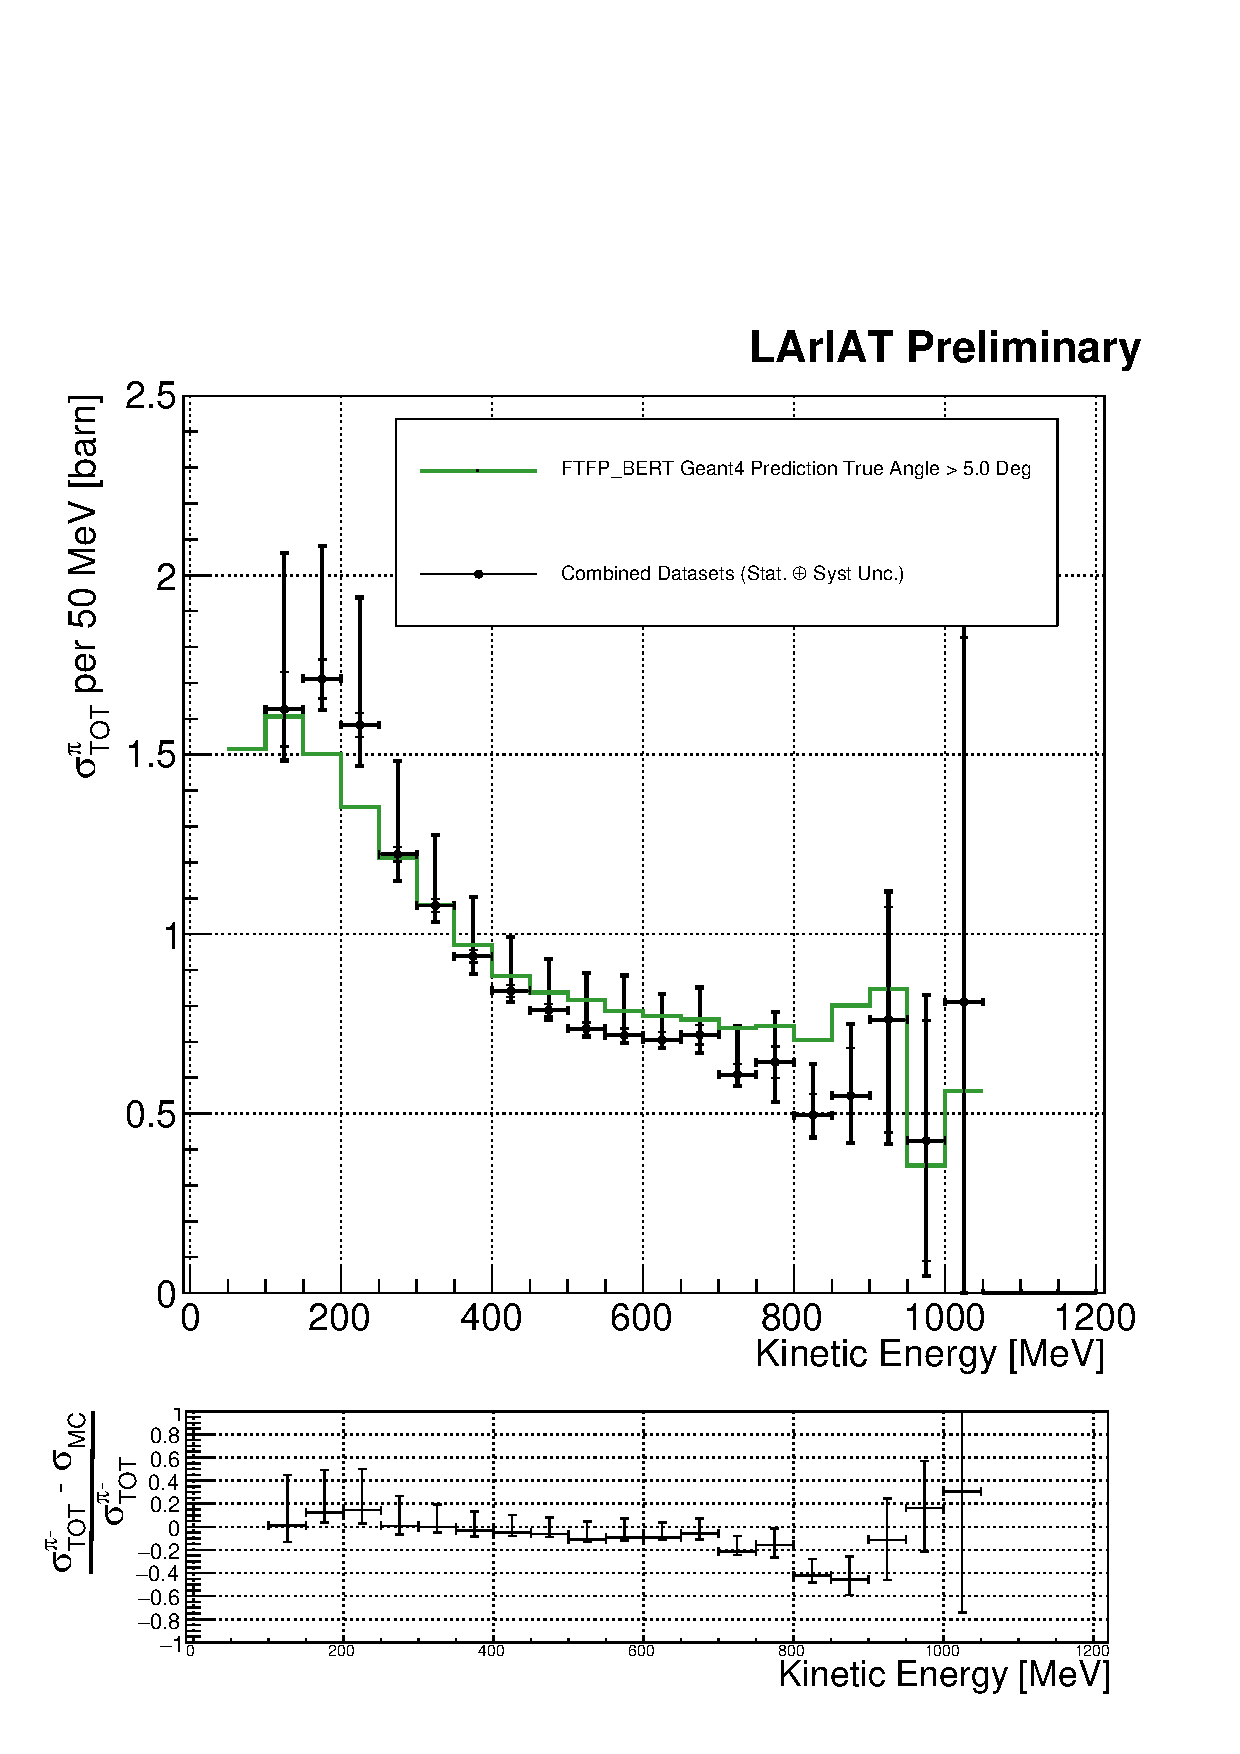
\includegraphics[width=0.48\textwidth]{Chapter-6/Images/TheRealMoneyPlot.pdf}
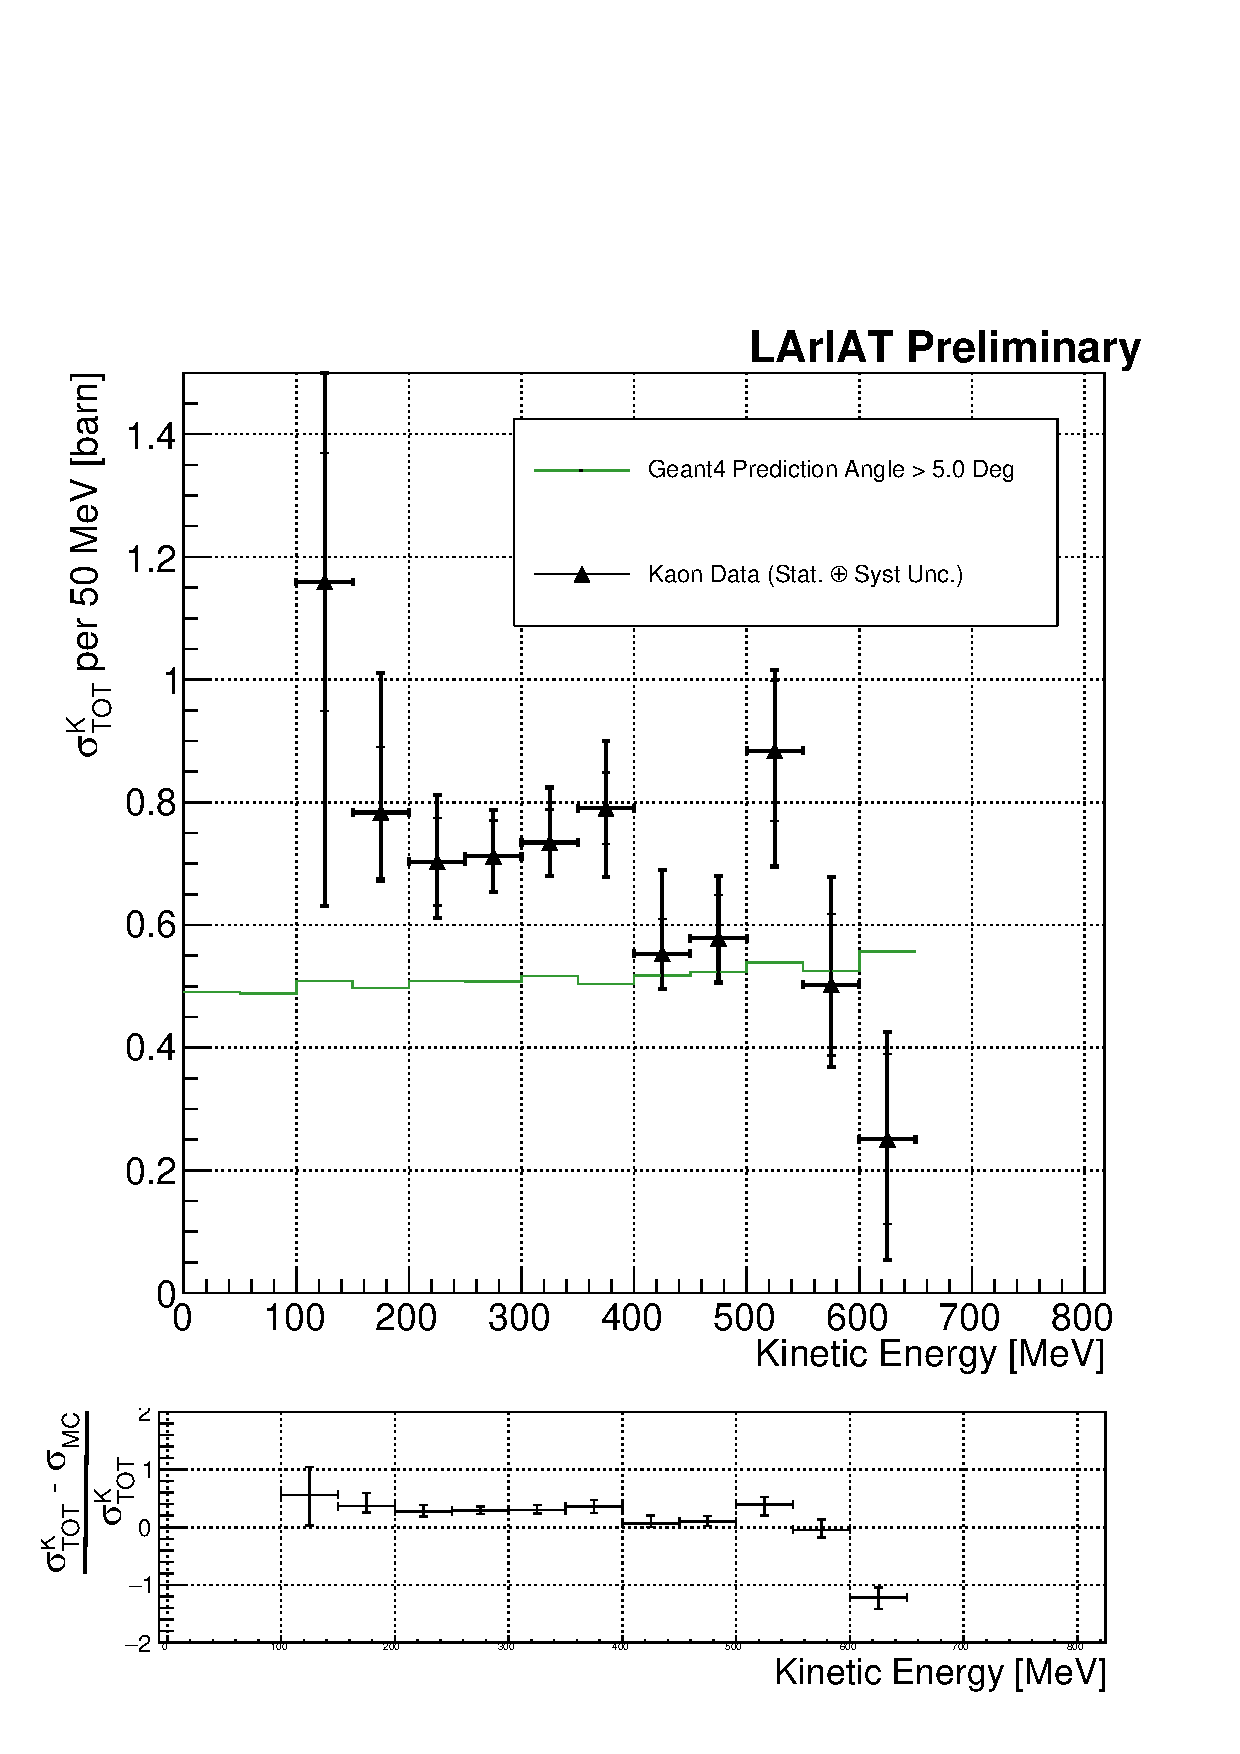
\includegraphics[width=0.48\textwidth]{Chapter-7/Images/TheMoneyPlotK.pdf}
\caption{\emph{Left:} ($\pi^-$-Ar) total hadronic cross section measurement for  scattering angles greater than 5$^\circ$ measured in the combined sample overlaid with the  Geant4 prediction (green). \emph{Right:} ($K^+$-Ar) total hadronic cross section for  scattering angles greater than 5$^\circ$ measured. The respective Geant4 prediction for the total hadronic cross section for angle scattering greater than 5$^\circ$ is displayed in green. } 
\label{fig:finalfinal}
\end{figure}



